\documentclass[12pt]{article}
\usepackage[spanish]{babel}
\usepackage{natbib}
\usepackage{url}
\usepackage[utf8x]{inputenc}
\usepackage{amsmath}
\usepackage{float}
\usepackage{subfig}
\usepackage{graphicx}
\graphicspath{{images/}}
\usepackage{parskip}
\usepackage{fancyhdr}
\usepackage{vmargin}
\usepackage{mathtools}
\usepackage{amssymb} 



\title{Actividad \#4: Ajuste de mìnimos cuadrados }							
\author{\Large Jesùs Valenzuela Nieblas\\}											
\date{\today} 

\makeatletter
\let\thetitle\@title
\let\theauthor\@author
\let\thedate\@date										
\makeatother

\pagestyle{fancy}

\lhead{\thetitle}
\cfoot{\thepage}

\begin{document}

%%%%%%%%%%%%%%%%%%%%%%%%%%%%%%%%%%%%%%%%%%%%%%%%%%%%%%%%%%%%%%%%%%%%%%%%%%%%%%%%%%%%%%%%%

\begin{titlepage}
	\centering
    \vspace*{.5cm}
     
\includegraphics[scale = 0.7]{logo}\\	% University Logo
    \textsc{\Large Universidad de Sonora}\\[1.0 cm]	% University Name
	\textsc{\Large División de Ciencias Exactas y Naturales}\\[.50 cm]
  	\textsc{\Large Licenciatura en Fìsica}\\[.5 cm]
  \textsc{\large Fìsica Computacional 1}\\[1.5 cm]				% Course Name
	
	{ \huge \bfseries \thetitle}\\

    \vspace*{3 cm}
	\begin{minipage}{\textwidth}
    \centering
    \theauthor
	\end{minipage}\\[3 cm]
	{\large \thedate}\\[2 cm]
 
	\vfill
	
\end{titlepage}

%%%%%%%%%%%%%%%%%%%%%%%%%%%%%%%%%%%%%%%%%%%%%%%%%%%%%%%%%%%%%%%%%%%%%%%%%%%%%%%%%%%%%%%%%

\section{Introducciòn}
Mínimos cuadrados es una técnica de análisis numérico enmarcada dentro de la optimización matemática, en la que, dados un conjunto de pares ordenados —variable independiente, variable dependiente— y una familia de funciones, se intenta encontrar la función continua, dentro de dicha familia, que mejor se aproxime a los datos (un "mejor ajuste"), de acuerdo con el criterio de mínimo error cuadrático.
\begin{figure}[H]
\centering
\includegraphics[]{ajus}
\end{figure}

En su forma más simple, intenta minimizar la suma de cuadrados de las diferencias en las ordenadas (llamadas residuos) entre los puntos generados por la función elegida y los correspondientes valores en los datos. Específicamente, se llama mínimos cuadrados promedio (LMS) cuando el número de datos medidos es 1 y se usa el método de descenso por gradiente para minimizar el residuo cuadrado. Se puede demostrar que LMS minimiza el residuo cuadrado esperado, con el mínimo de operaciones (por iteración), pero requiere un gran número de iteraciones para converger.

\section{Actividad a realizar}

En esta actividad se crearon dos programas que hacen un ajuste lineal y exponencial a un conjunto de datos sobre la temperatura del invierno en New York y la relaciòn presiòn-altitud respectivamente. 
 
 
 \section{Ajuste Lineal}
 EL siguiente còdigo fue el utilizado para hacer el ajuste lineal sobre los datos obtenidos de las temperaturas de invierno de la ciudad de New York de los años 1990-1999.
 \subsection{Còdigo}
 \begin{verbatim}
import numpy as np
import matplotlib.pyplot as plt
from scipy import optimize

datos=np.loadtxt('s48.txt')
x=datos[:,0]
y=datos[:,1]

fitfunc = lambda p, x: p[0]*x + p[1]
errfunc = lambda p, x, y: fitfunc(p, x) - y 
p0=[1,1]
p1, success=optimize.leastsq(errfunc, p0[:], args=(x,y))

time = np.linspace(x.min(), x.max(), 100)
plt.plot(x, y, "go", label="Datos") 
plt.plot(time, fitfunc(p1, time), "b-", label="Ajuste ineal")

plt.title("Temperatura del invierno en Nueva York (1990-1999)")
plt.xlabel("Año")
plt.ylabel("Temperatura")
plt.grid()
plt.legend()
plt.show()
\end{verbatim}
\subsection{ Resultado Obtenido}
 \begin{figure}[H]
\centering
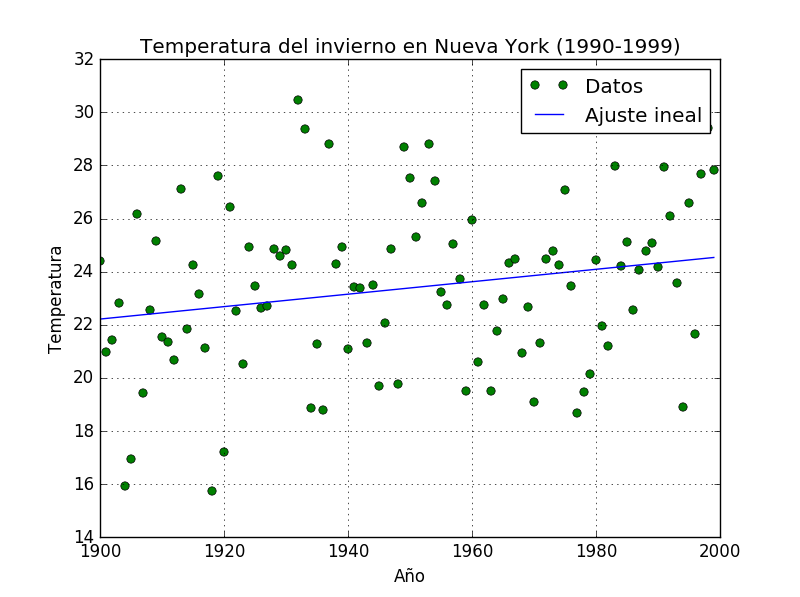
\includegraphics[scale=.5]{lineal}
\end{figure}
 
 
 \section{Ajuste Exponencial}
 El siguiente còdigo fue el utilizado para hacer un ajuste exponencial a los datos obtenidos de la relaciòn Presòn vs Altitud
\subsection{Còdigo}
\begin{verbatim}
import numpy as np
import matplotlib.pyplot as plt
from scipy import optimize

datos=np.loadtxt('s48.txt')
x=datos[:,0]
y=datos[:,1]

fitfunc = lambda p, x: p[0]*x + p[1]
errfunc = lambda p, x, y: fitfunc(p, x) - y 
p0=[1,1]
p1, success=optimize.leastsq(errfunc, p0[:], args=(x,y))

time = np.linspace(x.min(), x.max(), 100)
plt.plot(x, y, "go", label="Datos") 
plt.plot(time, fitfunc(p1, time), "b-", label="Ajuste ineal")

plt.title("Temperatura del invierno en Nueva York (1990-1999)")
plt.xlabel("Año")
plt.ylabel("Temperatura")
plt.grid()
plt.legend()
plt.show()
\end{verbatim}


\subsection{ Resultado Obtenido}
 \begin{figure}[H]
\centering
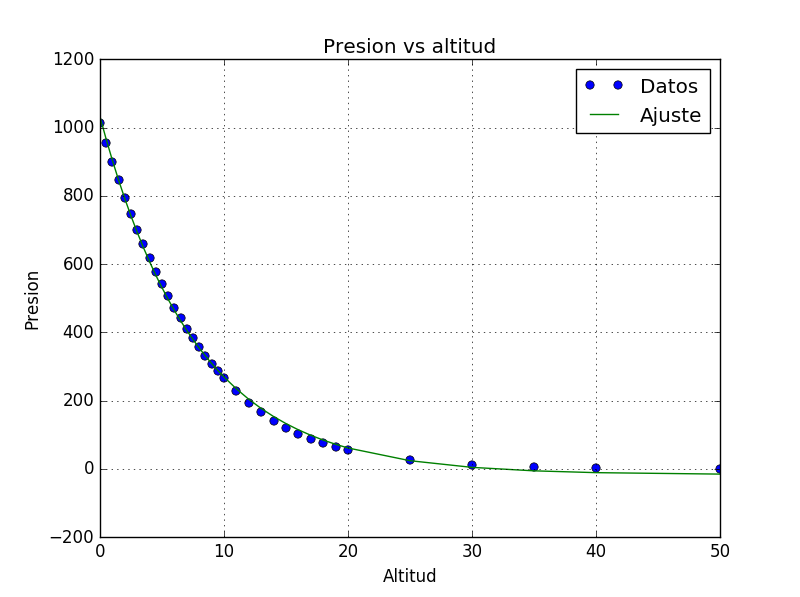
\includegraphics[scale=.5]{expo}
\end{figure}



\end{document}
